\begin{reviewer}
This paper proposed a novel approach to model transient power-temperature behavior considering process variation. This is a missing piece in statistical power/temperature analysis due to many reasons and technical difficulties. I think the proposed solution may still have some limitations and assumptions, but it has big contribution to the area, and one step closer to practical usage. Experiments are sufficient to validate the proposed framework. The paper is well written and organized as well.
\end{reviewer}
\begin{authors}
Thank you for the kind words.
\end{authors}

\begin{reviewer}
This is an interesting topic, so some of my comments are more like discussions:

1) Power consumption has two components: dynamic power and leakage power. Process variation mainly affects leakage power. I think that’s why the authors focus on the model for statistical leakage power. However, temperature and total power (dynamic and leakage) are highly correlated. Since this paper is focus on modeling transient power-temperature behavior, the accuracy of total power model is important. Dynamic power is related to the run-time operations. In Sec. VII, the dynamic power profiles are obtained by simulations of randomly generated via TGFF, applications defined by DAGs of tasks. Usually the simulation has a size limit, it will be nice to provide some details about how large scale of the chip can be.
\end{reviewer}
\begin{authors}
The workload to be analyzed is an input to our framework without any further restrictions: it is arbitrary and can come from an arbitrary source.
Therefore, it would not make much contribution to the paper if we performed, for example, cycle-accurate simulations of some real-life applications and used the output of these simulation as an input to our analysis.
Instead, our applications are generated randomly via TGFF.
Apart from a DAG, TGFF generates a set of tables that specify the execution time and dynamic power of each task for each processing element individually.
Then the simulation that we perform consists of a scheduling procedure of the DAG, which determines when and where each task should be executed (we employ a list scheduler for this purpose).
Once this has been decided, the corresponding dynamic power profile is constructed based on the tables provided by TGFF.
The output files of TGFF used in our experiments are available online.

In practice, of course, dynamic power profiles should be properly captured using adequate simulators capable of modeling the power dissipation.
In particular, the following interrelated tools are very frequently used for this purpose: SimpleScalar, PTscalar, gem5, McPAT, and Wattch.
As Reviewer~2 pointed out in the second comment, contemporary software packages can address ``[\ldots] fairly big size examples and circuits.''

\done{The input workload has been detailed further, Sec.~IV.}

\done{Practical aspects of the input workload have been outlined in Sec.~VII.}
\end{authors}

\begin{reviewer}
2) Question about the thermal model: The authors mentioned the following in Sec. IV-C: ``Given the thermal specification S of the system at hand (see Sec. IV), \ldots'' I’m interested in the modeling of thermal specification as well. But it seems that the authors are referring to the wrong Section (or should provide more details about sub-session?).
\end{reviewer}
\begin{authors}
The specification $\system$ is a shortcut for us to refer to all the information needed for the construction of an equivalent thermal RC circuit of the system.
The content of $\system$ is described in the second paragraph of Sec. IV, and it is specific to the way the RC circuit is obtained.
In our experiments, we utilize the block model of HotSpot v5.02 for this purpose.
$\system$ then reflects the configuration of HotSpot, which includes more than 60 parameters such as the chip thickness, silicon thermal conductivity, silicon specific heat, \etc\ Please refer to ``Temperature-aware Microarchitecture: Modeling and Implementation'' by K. Skadron \etal\ for further details.

\done{The reference to $\system$ from Sec.~V-C has been improved.}

\done{The content of $\system$ has been detailed further, Sec.~IV.}

\done{Two references, namely, [Kreith, 2000] ([22] in the previous version) and [HotSpot] ([31] in the previous version), have been replaced by [Skadron, 2004], mentioned above, which is more concrete and well suited for the discussions in the paper.}
\end{authors}

\begin{reviewer}
In Sec. III, the authors mentioned that this framework works for electronic systems with temperature profiles. Is that chip level? Architecture level? If it’s chip level, the cooling system is not settled yet, so it’s hard to have a final temperature profile;
\end{reviewer}
\begin{authors}
The thermal modeling considered in this paper is at the architecture/system level.
The cooling system is assumed to be settled in order to construct an adequate thermal RC circuit.
Therefore, the thermal package is included in the thermal model, as mentioned in the second paragraph of Sec.~IV.
To elaborate, the thermal package in the experimental results consists of three layers: the thermal interface material, heat spreader, and heat sink.
Unfortunately, due to the shortage of space, we no longer have an illustration of such a circuit with a thermal package in the paper.
However, we would like to give it here.
\begin{figure}[!h]
  \centering
  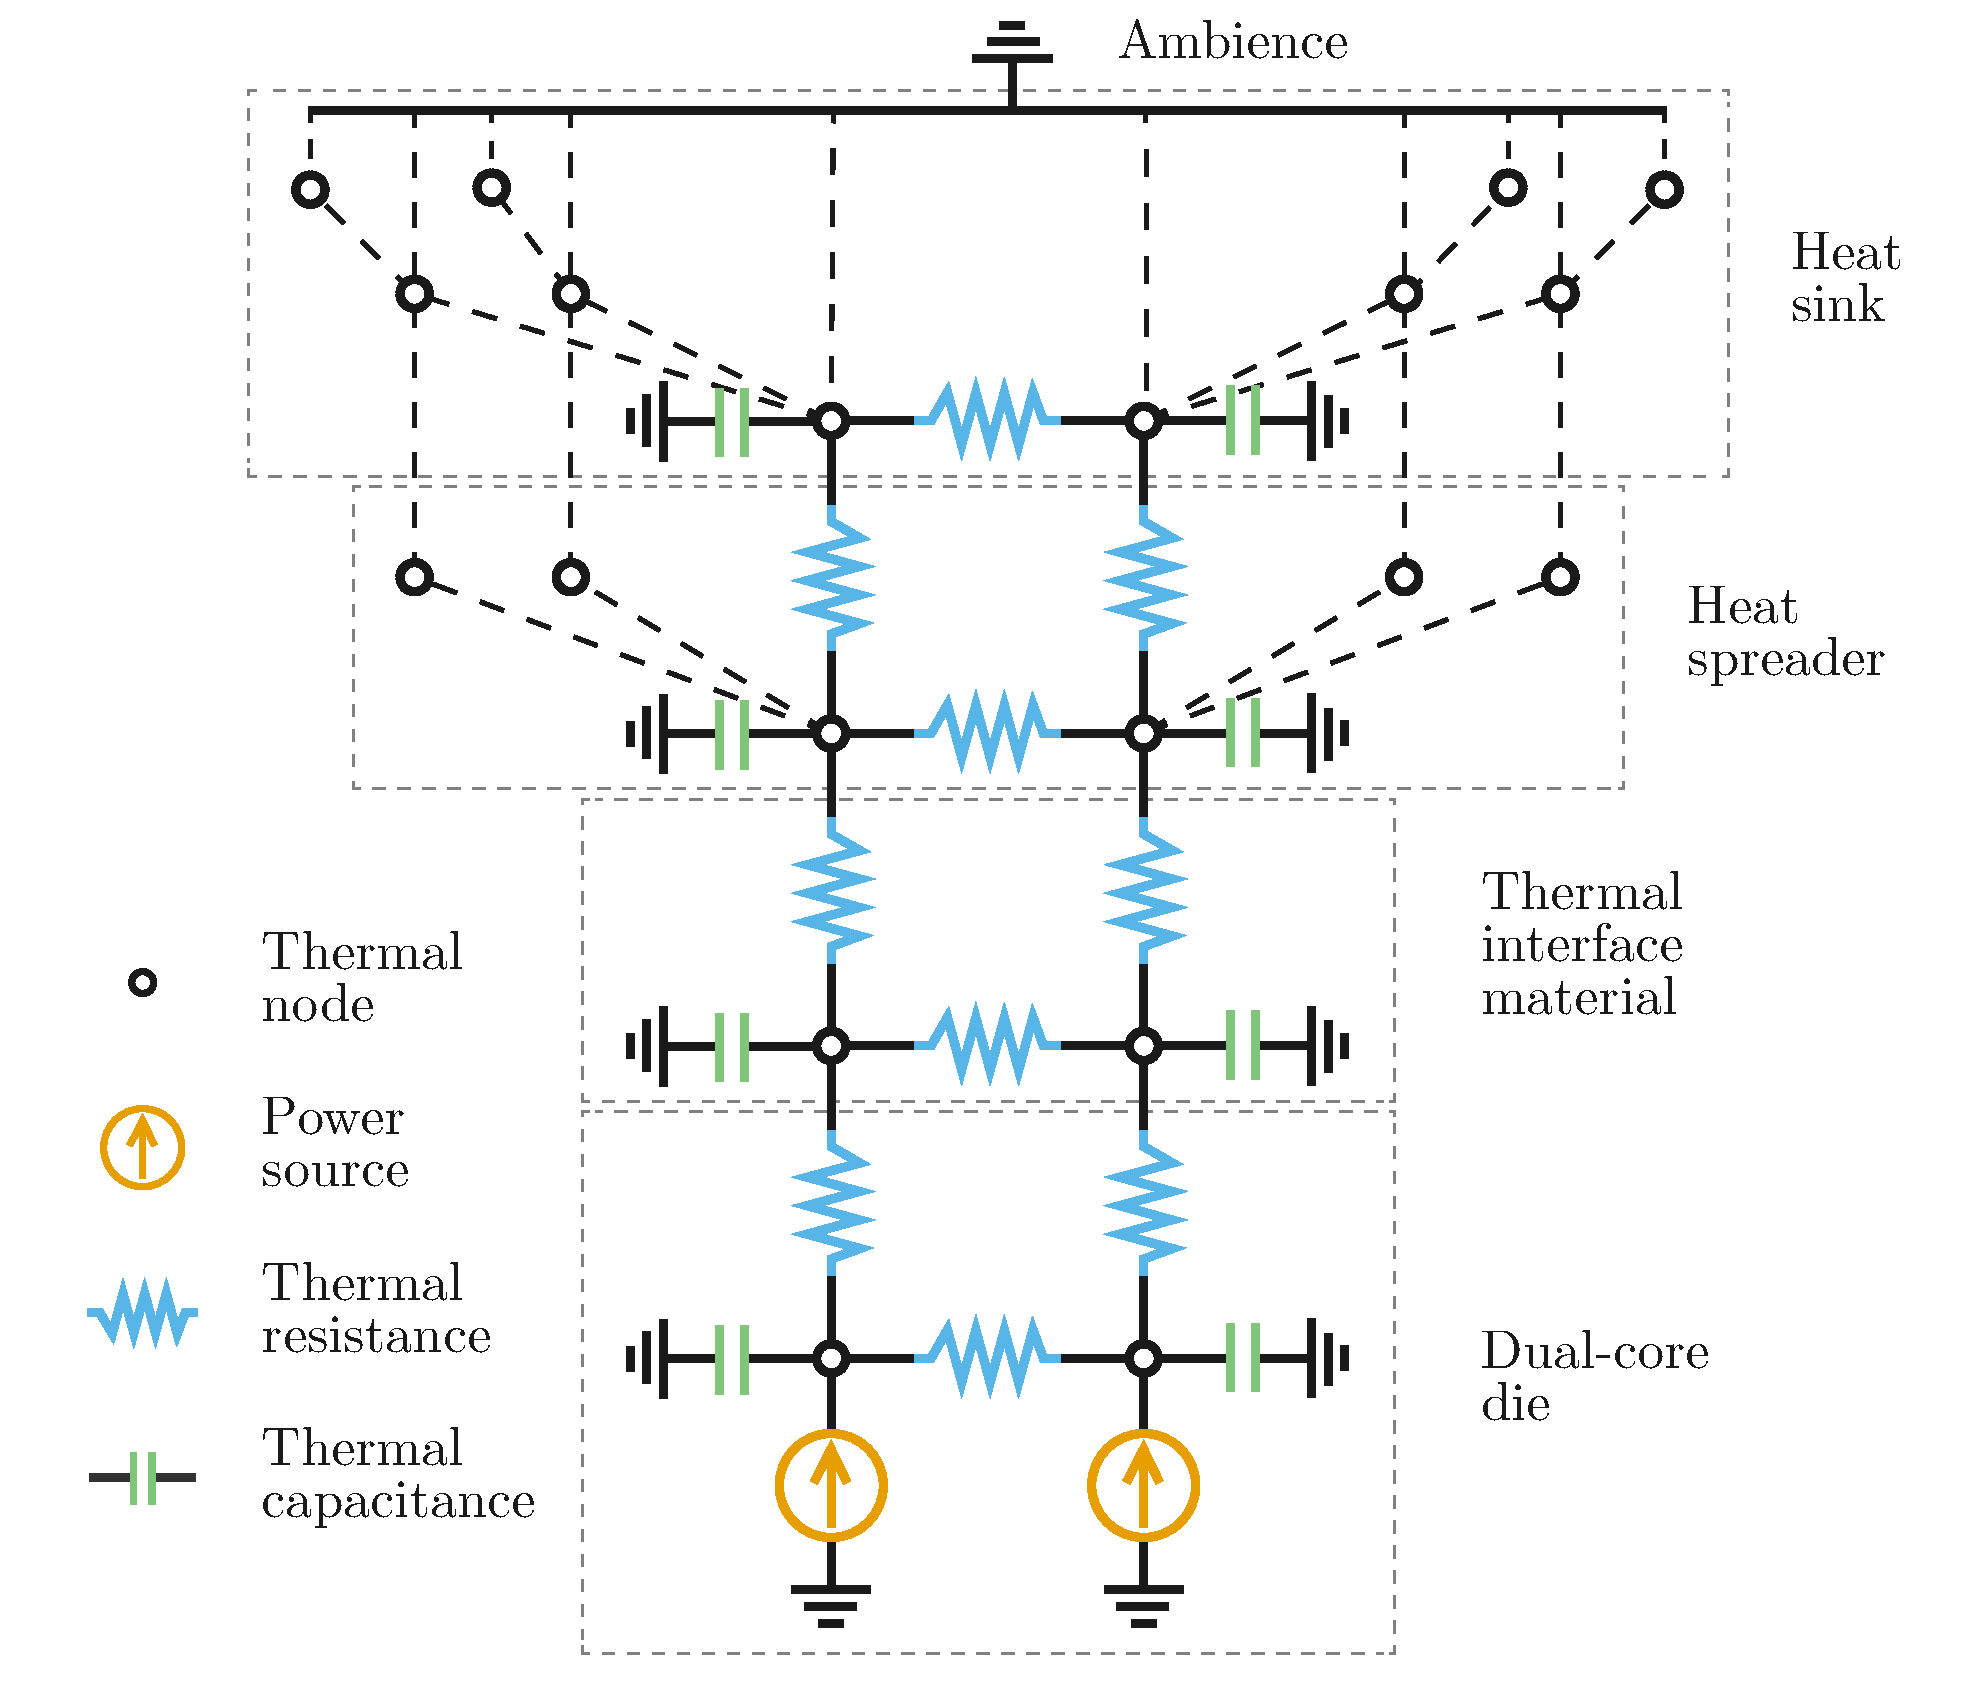
\includegraphics[width=0.5\linewidth]{include/assets/circuit.pdf}
  \vspace{-0.5em}
  \caption{A simplified thermal RC circuit for a dual-core platform.}
  \flabel{circuit}
\end{figure}

The top three dashed boxes in \fref{circuit} correspond to the aforementioned three layers.

\done{The system-level scope of the paper has been emphasized in Sec.~IV.}
\end{authors}

\begin{reviewer}
If it’s architecture level, there might be multiple chips involved with different statistical power behaviors, I’m curious about how the proposed method works in this situation.
\end{reviewer}
\begin{authors}
The source of uncertainty considered in this work is process variation.
At the design stage, the process parameters of a yet-to-be-fabricated chip are random variables.
Once the chip has been fabricated, these parameters take particular values and remain fixed hereafter, \ie, the process parameters of this particular chip become deterministic.
Thus, a \emph{fabricated} chip does \emph{not} exhibit any statistical behavior; the behavior is deterministic.
However, since this behavior is unknown at the design stage, the power/temperature profiles are stochastic for the designer, and our framework provides with the tools to characterizes all possible outcomes of these uncertain profiles.

\done{The above discussion has been included in Sec.~IV.}
\end{authors}

\begin{reviewer}
3) On Fig 1, it will be nice to use different line shapes as well. When the paper is printed black/white, it’s hard to tell the color difference.
\end{reviewer}
\begin{authors}

\done{Fig.~1 have been adapted for printing in grayscale.}

\done{The same issue has been addressed regarding Fig.~3, Fig.~4, Fig.~5, and Fig.~6.}
\end{authors}
